\chapter{Mathematical Models for Combustion}\label{chap:model}

Mathematicals models for predicting combustion phenomena stem from the
from the compressible, reacting, Navier-Stokes equations~\cite{PoinsotVeynante3ed}. In absence
of dominant acoustic phenomena, an asymptotic analysis yields the low
Mach number approximation that is very typical in combustion
modeling~\cite{Muller,Codina,PoinsotVeynante3ed,Kuo} --- this system of partial differential equations is
described in Section~\ref{sec:lowmach}. Appendix~\ref{chap:app}
illustrates the asymptotic analysis for the non-reacting equations. One-dimensional models are
also frequently used for studying freely propagating flames --- these
models are discussed in Section~\ref{sec:1d}. Such
scenarios arise are commonly used experimentally for measuring laminar
speeds in experiments~\cite{}.

\section{Governing Equations}\label{sec:lowmach}

Given a multicomponent gas over the domain of interest, we make the
following assumptions: the gas can be modeled as a continuum, the
ideal gas law is applicable and valid, the gas behaves as a Newtonian
fluid, the thermodynamic pressure
is constant (follows from the low Mach number assumption), the Dufor
effect is neglible (energy transport due to mass fraction gradients),
the Soret effect is neglible (mass transport due to thermal
gradient), and radiative heating is negligible. Then, the following system of partial differential
equations holds~\cite{PoinsotVeynante3ed}:

\begin{equation}
\begin{aligned}
\nabla \cdot \bu &= \frac{1}{T}\frac{DT}{Dt} - \frac{1}{M}\frac{DM}{dt} \\ %- \frac{1}{p^0} \frac{dp^0}{dt} \\
\rho \frac{D Y_s}{D t} &= \nabla \cdot \boldsymbol{j}_s + \dot{\omega}_s \quad s = 1 \dots N_s \\
\rho \frac{D\bu}{Dt} &= -\nabla p + \nabla \cdot \mathbf{\tau} + \rho \boldsymbol{g} \\
\rho c_p \frac{DT}{Dt} %- \frac{dp^0}{dt}
&= \nabla \cdot \left(k \nabla T \right) - \sum_s h_s \dot{\omega_s} -
\nabla T  \cdot \left( \sum_{s} c_{p,s} \boldsymbol{j}_s \right) +
\sum_{s} \rho \boldsymbol{g} \cdot \boldsymbol{j}_s \\
%\frac{dp^0}{dt} \int_{\Omega} \frac{1}{\gamma - 1} \; d\mathbf{x} &= -p^0 \int_{\Omega} \frac{\gamma}{\gamma - 1} \nabla \cdot \mathbf{u} \; d
%\mathbf{x} + \int_{\partial \Omega} k \nabla T \cdot \mathbf{n} \; dS \\
p^0 &= \rho R T
\end{aligned}
\end{equation}
where $\bu$ is the mixtured averaged velocity of the gas, $T$ is the temperature of the
gas, $M$ is the mixture molar mass, $\rho$ is the mixture density,
$Y_s$ is the mass fraction of species $s$ with a total of $N_s$ species, $\boldsymbol{j}_s$ is the
mass diffusion flux of species $s$, $\dot{\omega}_s$ is the mass of
species $s$ generated due to chemical reactions, $p$ is the
hydrostatic pressure, $\tau$ is the viscous stress tensor,
$\boldsymbol{g}$ is acceleration due to gravity, $c_p$ is the mixture
specific heat, $k$ is the mixture thermal conductivity, $h_s$ is the
enthalpy of the gas, $c_{p,s}$ is the specific heat of species $s$,
$p^0$ is the thermodynamic pressure, and $R$ is the gas constant of
the mixture.

The species mass fraction $Y_s$ is defined as
%
\begin{equation}
  Y_s = \frac{\rho_s}{\rho}
\end{equation}
%
where $\rho_s$ is the density of species $s$.
The mixture molar mass $M$ is given as
%
\begin{equation}
  \frac{1}{M} = \sum_{s=1}^{N_s} \frac{Y_i}{M_i}
\end{equation}
%
where $M_i$ is the molar mass of species $i$.
%
For a Newtonian fluid, the viscous stress tensor is given as
%
\begin{equation}\label{eq:stress_tensor}
  \tau = \mu\left(\nabla\bu + \nabla^{T}\bu\right) -\frac{2}{3}\mu \left(\nabla\cdot\bu\right)\boldsymbol{I}
\end{equation}
%
where $mu$ is the viscosity of the gas mixture.
%
Species thermodynamic quantities are computed using table lookup from the NASA
CEA tables~\cite{CEATables}.
Mixture quanties are then just a sum of the species
quantity weighted by the species mass fraction, e.g.
%
\begin{equation}
  c_p = \sum_{s=1}^{N_s} Y_s c_{p,s}
\end{equation}
%

The discussion of the mass diffusion flux follows that of~\cite{Kee}.
The species mass diffusion flux, $\boldsymbol{j}_s$, is defined in terms
of the species diffusion velocity, $\boldsymbol{V}_s$. In particular,
let $\tilde{\boldsymbol{V}}_s$ be the average velocity of species $s$
relative to a fixed reference frame. Then, the mixture averaged
velocity, $\bu$, is
%
\begin{equation}
  \bu = \sum_{s=1}^{N_s} Y_s \tilde{\boldsymbol{V}}_s
\end{equation}
%
and the species velocity, $\boldsymbol{V}_s$, is
%
\begin{equation}
  \boldsymbol{V}_s = \tilde{\boldsymbol{V}}_s - \bu
\end{equation}
%
Then, then mass diffusion flux is
%
\begin{equation}
  \boldsymbol{j}_s = \rho_s \left( \tilde{\boldsymbol{V}}_s - \bu
  \right) = \rho Y_s \boldsymbol{V}_s
\end{equation}
%
We assume a Fick's law relationship for the mass diffusion flux
$\boldsymbol{j}_s$. For the ``full multicomponent'' model, this yields
a coupled system of equations to solve at every point in
space. Instead, for computational simplicity, we assume a
``mixture-averaged'' model. The primary assumption here is that
species velocity is the \emph{same} for every species, i.e.
%
\begin{equation}
  \boldsymbol{V}_j - \boldsymbol{V}_k = 0, \quad j \ne k
\end{equation}
%
Under this assumption, the mass diffusion flux is
%
\begin{equation}
  \boldsymbol{j}_s = -\rho D_s \nabla Y_s
\end{equation}
%
where
%
\begin{equation}
  \frac{1}{D_s} = \sum_{t\ne s} \frac{X_t}{\mathcal{D}_{st}} +
  \frac{X_s}{1-Y_s} \sum_{t\ne s} \frac{Y_t}{\mathcal{D}_{st}}
\end{equation}
%
where $\mathcal{D}_{st}$ are the binary diffusion coefficients between
species $s$ and $t$ and $X_s$ is the mole fraction of species $s$. The
construction of the binary diffusion coefficents is discussed in
Section~\ref{sec:species-trans}


The remaining mixture transport properties are computed using the
Wilke mixing rule~\cite{Wilke} based on the values of species
quantities. In particular, the viscosity is given by
%
\begin{equation}
\mu = \sum_{s=1}^{N_s} \mu_s \frac{X_s}{\phi_s}
\end{equation}
%
and the thermal conductivity is given by
%
\begin{equation}
k = \sum_{s=1}^{N_s} k_s \frac{X_s}{\phi_s}
\end{equation}
%
where $\phi_s$ is given by
%
\begin{equation}
\phi_s = \sum_{t=1}^{N_s} X_t \frac{ \left(1 +
  \sqrt{\frac{\mu_s}{\mu_t}}\sqrt[4]{\frac{M_t}{M_s}}\right)^2}{\sqrt{8\left(
1+ \frac{M_s}{M_t}\right)}}
\end{equation}
%
The species properties $\mu_s$ and $k_s$ are discusste in
Section~\ref{sec:species-trans}.

%=======================================================================
% Kinetics
%=======================================================================
The rate of production/destruction of the individual species,
$\dot{\omega}_s$, is required to close the species continuity
equations.  These rates are computed using principles from the theory
of chemical kinetics. In particular, the net production rate of each
species is determined by a set of $r$ reactions.
Each of these $r$ reactions is of the canonical form
\begin{align}
  \mathcal{R}_r &= \mathcal{R}_{b,r} - \mathcal{R}_{f,r} \\ &= k_{b,r}
  \prod_{s=1}^{N_s} \left(\frac{\rho_s}{M_s}\right)^{\beta_{sr}} -
  k_{f,r} \prod_{s=1}^{N_s}
  \left(\frac{\rho_s}{M_s}\right)^{\alpha_{sr}}
\end{align}
where $k_{fr}$ and $k_{br}$ are the forward and backward reactions
rates, respectively while $\alpha_{sr}$ and $\beta_{sr}$ are the
stoichiometric coefficients for reactants and products of species $s$.
The source terms can then be expressed in the canonical form
%
\begin{equation}
  \dot{\omega}_s = M_s \sum_{r=1}^{nr}\left(\beta_{sr}-\alpha_{sr}\right)\left(\mathcal{R}_{f,r} - \mathcal{R}_{b,r}\right)
\end{equation}
%
where $nr$ is the number of reactions.
The forward rate coefficients are expressed in a modified Arrhenius form as
%
\begin{equation}\label{eq:arrhenius}
%  \label{eq:k_fr}
  k_{f,r}\left(T\right) = A_{r} T^{\eta_r} \exp \left(-E_{r}/RT\right)
\end{equation}
%
where
$C_{fr}$ is the reaction rate constant, $\eta_r$ is the so-called pre-exponential factor, and $E_{ar}$ is the activation energy.
The three constants are determined from curve fits to experimental data.

%
The backward rate coefficient can be found using the principle of detailed balance, which states
\begin{equation}
  \label{eq:k_br}
  K_{eq,r} = \frac{k_{f,r}\left(T\right)}{k_{b,r}\left(T\right)}
\end{equation}
%
where $K_{eq}$ is the equilibrium constant and may be obtained through Gibbs' free energy minimization. Specifically, for reaction $r$ we have
%
\begin{equation}
  \label{eq:k_eq}
  K_{eq,r}\left(T\right) =
  \left(\frac{P_0}{RT}\right)^{\nu_r}\exp\left[-\sum_s\left(\beta_{sr}-\alpha_{sr}\right)\left(\frac{H^\circ_s}{RT} - \frac{S^\circ_s}{R}\right)\right]
\end{equation}
%
where $P_0= 10^5 [Pa]$ is the standard reference pressure,
%
\begin{equation}
  \nu_r \equiv \sum_s\left(\beta_{sr}-\alpha_{sr}\right)
\end{equation}
%
and the normalized enthalpy, $H^{\circ_s}/RT$, and entropy, $S^{\circ_s}/R$, data are available from curve fit data~\cite{CEATables}.

%=======================================================================
% Species Transport Properties
%=======================================================================
\section{Species Transport Properties}\label{sec:species-trans}

In this section, we describe the models that are used to compute the
species transport properties. First, we described viscosity, then
thermal conductivity, and then the bimolecular diffusion. The
development is based on the kinetic theory of gasses and follows that of~\cite{Kee}, but can be traced back to
Hirschfelder et al~\cite{Curtiss}.

%=======================================================================
% Species Viscosity
%=======================================================================
\subsection{Viscocity}
The viscocity of the species is given by the following formula
\begin{equation}
\mu_s = \frac{5}{16}\sqrt{\frac{m_s k_B T}{\pi}}\frac{f_n}{{\sigma_s}^2   \Omega^{(2,2^*)}}
\end{equation}
%
where $m_s$ the molecular mass of the species (kg), $\sigma_s$ is the
Lennard-Jones potential diameter associated to the species $m_s$,
$k_B$ is the Boltzmann constant, $\Omega^{(2,2^*)}$ is the value of
the dimensionless integrated integral value determined by a quadratic
interpolations of tables based on Stockmayer potntials given in from
Monchick and Mason\cite{Monchick}. For the hard sphere approximation,
$f_n = 1$.  There are three species of primary interest here: $O$,
$O_2$ and $O_3$. We have varied temperature from 300 K to 2700 K and
plotted the species viscocity for all the three species. The $\sigma$
values and constants for dimensionless collision number are taken from
GriMech~3.0~\cite{gri}.
\begin{figure}[H]
  \centering
  \includegraphics[scale=0.5]{figs/viscmodel.png}
   \caption{Species viscocity for $O$, $O_2$ and $O_3$.}
\end{figure}


%=======================================================================
% Species Thermal Conductivity
%=======================================================================
\subsection{Thermal Conductivity}

The thermal conductivity of species $i$ is given by
\begin{eqnarray*}
k_i &=& k_i^{(\textnormal{rot})} + k_i^{(\textnormal{trans})} + k_i^{(\textnormal{vib})} \\
k_i &=& \frac{\eta_i}{M_i} \left(
                        C_{v,i}^{(\textnormal{trans})} k_i^{(\textnormal{trans})} + C_{v,i}^{(\textnormal{rot})} k_i^{(\textnormal{rot})}+ C_{v,i}^{(\textnormal{vib})}  k_i^{(\textnormal{vib})}
                                          \right)
\end{eqnarray*}
with
%%
\begin{eqnarray*}
k_{v,i}^{(\textnormal{vib})}   & =& \rho_i \frac{D_{i,i}}{\eta_i} \\
k_{v,i}^{(\textnormal{rot})}   & =& \rho_i \frac{D_{i,i}}{\eta_i}\left(1 + \frac{2}{\pi}\frac{A}{B}\right) \\
k_{v,i}^{(\textnormal{trans})}   & =&  \frac{5}{2} \left(1 - \frac{2}{\pi}\frac{C_{v,i}^{(\textnormal{rot})}}{C_{v,i}^{(\textnormal{trans})}}\frac{A}{B}\right)
\end{eqnarray*}
%
and
%
\begin{eqnarray*}
  A & = & \frac{5}{2} -  \rho_i \frac{D_{i,i}}{\eta_i}  \\
  B & = & Z_{rot} + \frac{2}{\pi} \left(\frac{5}{3}\frac{C_{v,i}^{(\textnormal{rot})}}{R} + \rho_i \frac{D_{i,i}}{\eta_i}\right)
\end{eqnarray*}
%
 the rotational relaxation number is given by
\begin{equation}
Z_{rot,i}(T) = Z_{rot,i}(298)\frac{F(298)}{F(T)}
\label{thermal_cond:Zrot}
\end{equation}
 with the function $F$ defined as
\begin{equation}
F(T) = 1 + \frac{\pi^{\frac{3}{2}}}{2}\sqrt{\left(\frac{\epsilon_i}{k_B T}\right)}
         + \left(\frac{\pi^2}{4} + 2\right)\left(\frac{\epsilon_i}{k_B T}\right)
         + \pi^{\frac{3}{2}}\left(\frac{\epsilon_i}{k_B T}\right)^{\frac{3}{2}}
\end{equation}
%
The individual species conductivities composed of translational,
rotational and vibrational contribution was given by
Warnatz~\cite{Warnatz}. The temperature dependence given in rotational
relaxation number expression is given by Parker~\cite{Parker} and Brau
and Jonkman~\cite{Jonkman}. The specific heats are given by the NASA CEA
thermodynamic tables~\cite{CEATables}.  We have varied temperature from 300 K to 2700 K
and plotted the thermal conductivity for all the three
species. The $\sigma$ values and constants for dimensionless collision
number are taken from GriMech 3.0~\cite{gri}.

\begin{figure}[H]

\subfloat[Thermal Conductivity for $O$\label{fig:species-k-1}]{%
     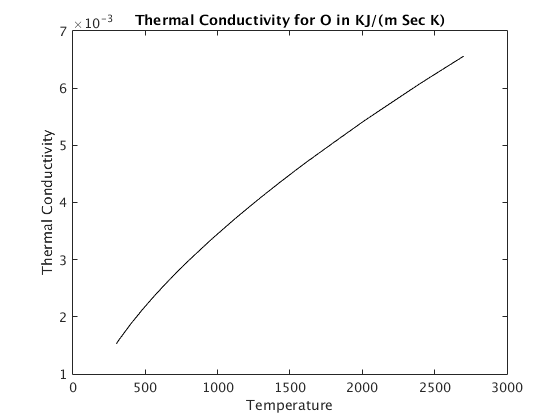
\includegraphics[scale=0.5]{figs/tcO.png}
    }
\subfloat[Thermal Conductivity for $O_2$ and $O_3$ \label{fig:species-k-2}]{%
     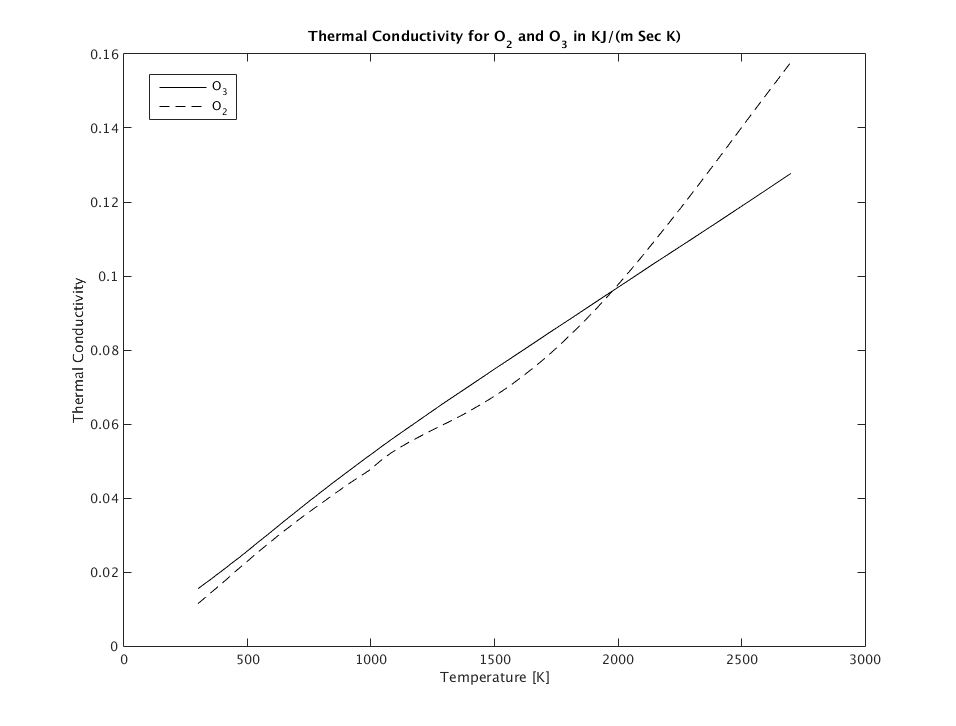
\includegraphics[scale=0.5]{figs/tco2_03.png}
    }

    \caption{Species thermal conductivity for $O$, $O_2$ and $O_3$.}
\end{figure}

%=======================================================================
% Bimolecular Diffusion
%=======================================================================
\subsection{Bimolecular Diffusion}
 The molecular binary diffusion model is
computed from kinetics theory, assuming an ideal gas. The molecular binary diffusion\cite{Curtiss} coefficient ($m^2 s^{-1}$ ) is given by:
%
\begin{equation}
  \mathcal{D}_{ij} = \frac{3}{16}\sqrt{\frac{2 k_B^3 T^3}{\pi m_{ij}}}\frac{f_n}{{ P \sigma_{ij}}^2   \Omega^{(1,1^*)}}
\end{equation}
with  the reduced mass
\begin{equation}
m_{ij} = \left\{\begin{array}{l@{\qquad}l}
                \frac{m_i m_j}{m_i + m_j} &  i \neq j \\
                m_i                                  & i=j
                    \end{array}
              \right.
\end{equation}

$\sigma_{ij}$ is the Lennard-Jones collision diameter between species $i$ and $j$:
\begin{equation}
\sigma_{ij} = \frac{1}{2}\left(\sigma_i + \sigma_j\right) \xi^{-\frac{1}{6}}
\end{equation}

 and $\Omega^{(1,1^*)}$ the integrated collision interval,
fitted from the tables given in Monchick and Mason \cite{Monchick}. We
have varied temperature from 300 K to 2700 K and plotted the diffusion
coefficients for all the combinations of the three species.
The $\sigma$ values and constants for dimensionless collision number
are taken from GriMech~3.0~\cite{gri}.


\begin{figure}[H]

\subfloat[Binary diffusion coefficients for $O_2-O_2$ and $O-O_2$ \label{fig:species-D-1}]{%
     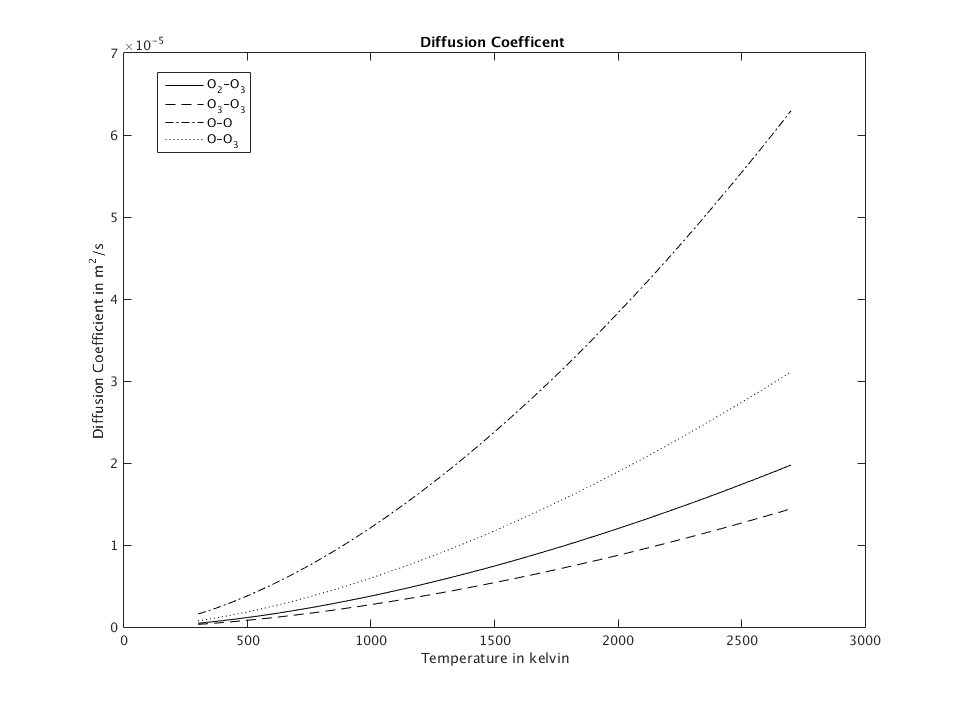
\includegraphics[scale=0.3]{figs/other.png}
    }
 \subfloat[Binary diffusion coefficients for other \label{fig:species-D-2}]{%
     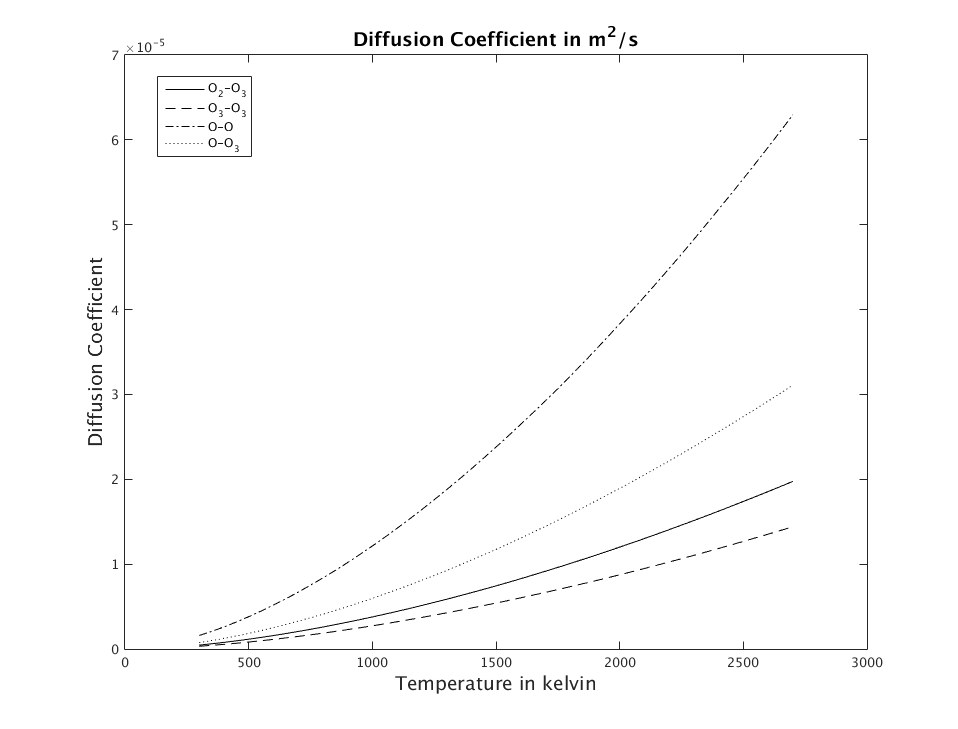
\includegraphics[scale=0.3]{figs/allinone.png}
    }

    \caption{Binary diffusion coefficients for $O_2-O_2$, $O_2-O_3$, $O_3-O_3$, $O-O$, $O-O_2$ and $O-O_3$}
\end{figure}


We also show examples of the final mixture transport properties for a
variety of mixtures. We have varied temperature from 300 K to 2700 K and plotted the
mixture viscocity V/s Temperature for all the three species.  We have
considered three cases- behind the flame where concentration of
$O_3$, $O_2$, and $O$ are taken to be .53, .47, and 0,
respectively. The second case is inside of the flame with
concentrations given by 0.5, 0.4, and 0.1, respectively. The third
case is the behind the flame where ozone and atomic oxygen are absent and
there will be only $O_2$. The $\sigma$ values and constants for
dimensionless collision number are taken from GriMech 3.0\cite{gri}.

\begin{figure}[H]

\subfloat[Mixture viscocity behind the flame. \label{fig:mix-visc}]{%
     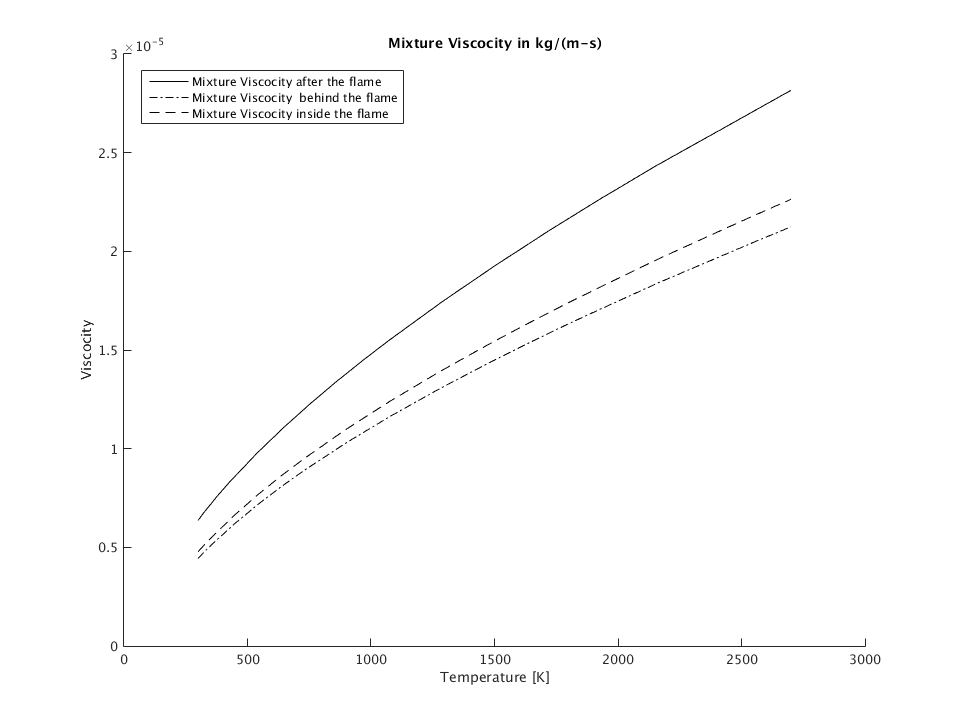
\includegraphics[scale=0.5]{figs/all_in_one.png}
    }

    \caption{Mixture Viscocity behind, inside, and after the flame}
\end{figure}

\begin{figure}[H]

\subfloat[Mixture Diffusion coefficient for $O_3$ and $O_2$ \label{fig:mix-diff1}]{%
     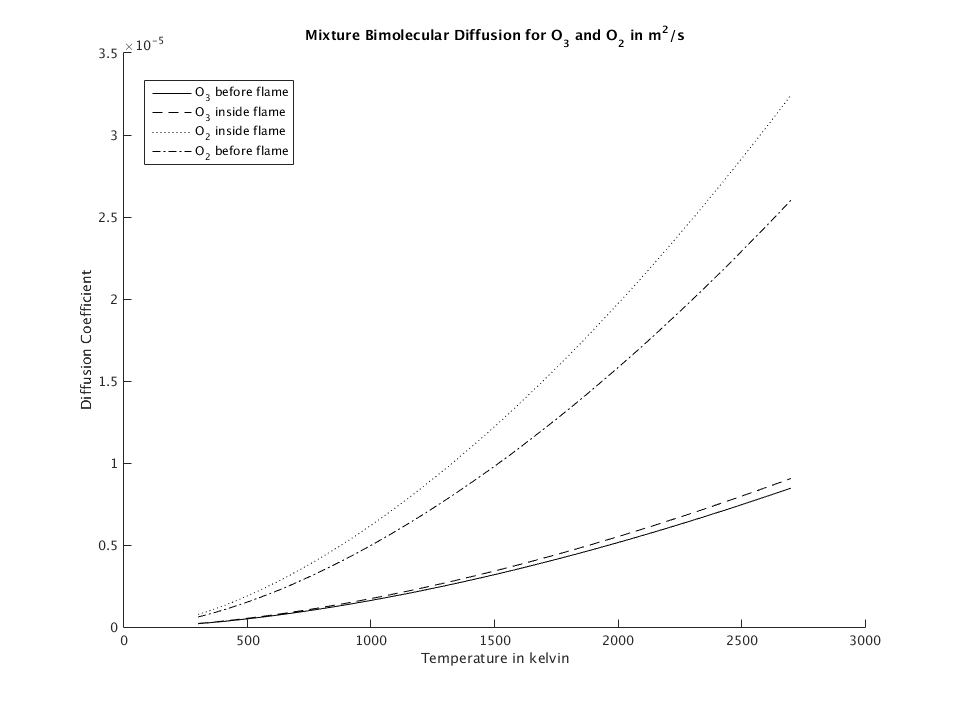
\includegraphics[scale=0.32]{figs/mixdiffusionO2O3.png}
    }
  \subfloat[Mixture Diffusion coefficient for $O$ inside the flame\label{fig:mix-diff2}]{%
         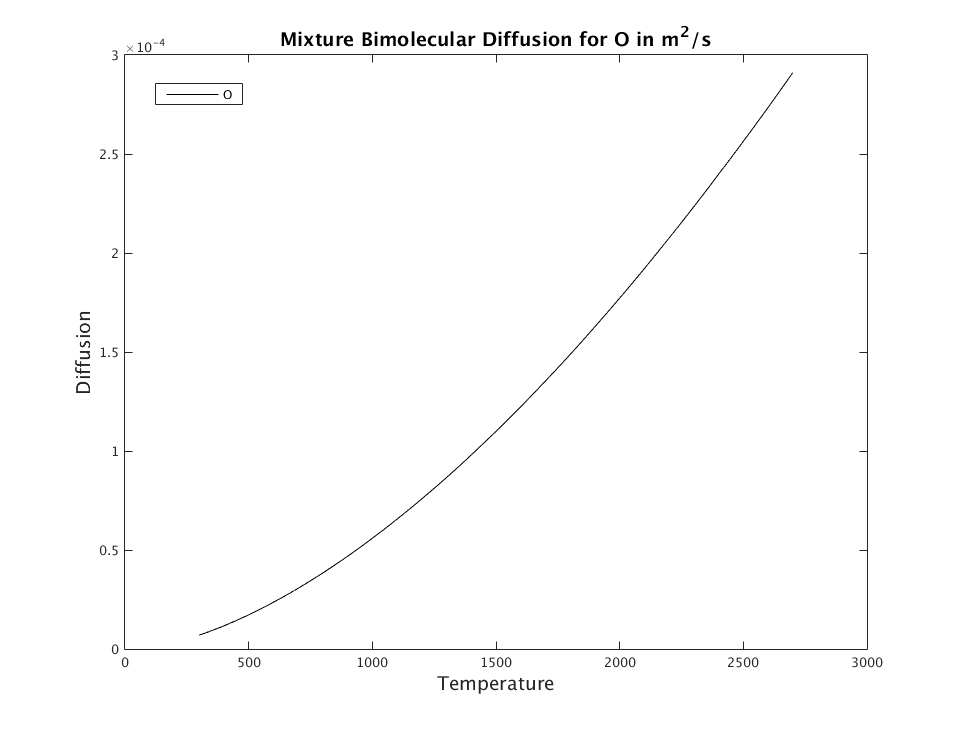
\includegraphics[scale=0.5]{figs/mixturediffusionO_inflame.png}
        }

    \caption{Mixture Diffusion coefficient}
\end{figure}

\begin{figure}[H]

\subfloat[Mixture thermal conductivity \label{fig:mix-cond}]{%
     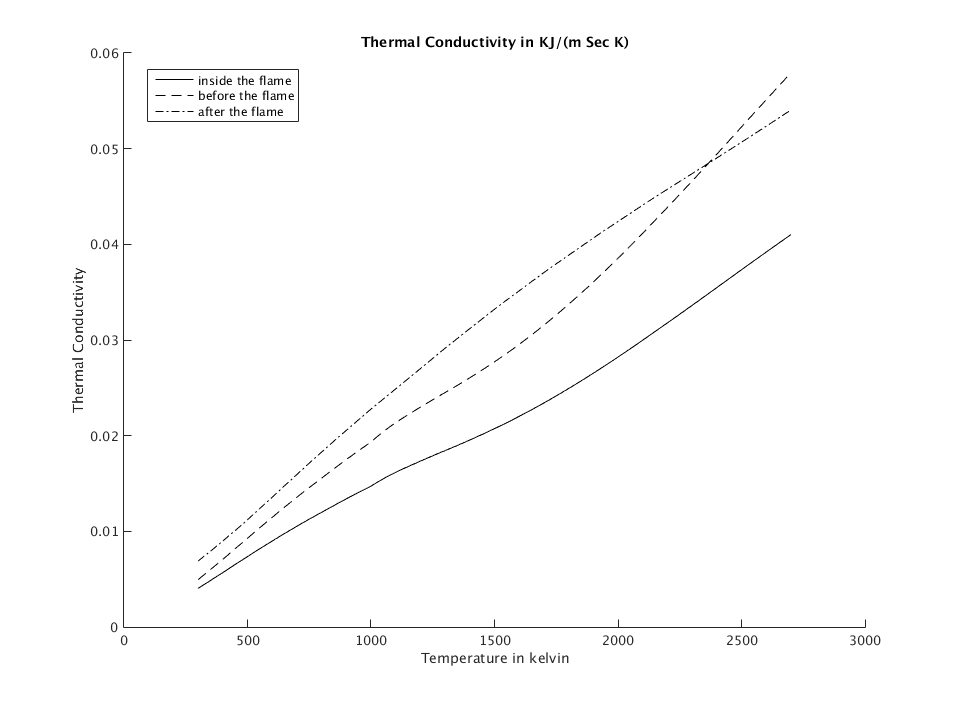
\includegraphics[scale=0.5]{figs/mixtherm.png}
    }

    \caption{Mixture thermal conductivity}
\end{figure}


%% \subsection{Mixture Model}
%%  The Wilke\cite{Wilke} formula and modified by Bird et al \cite{Bird} for viscosity, independent of the viscocity model, is
%% \begin{equation}
%% \eta_{\textnormal{mixture}} = \sum_{s=1}^{n} \frac {x_i \eta_i}{\sum_{j=1}^{n} x_j \Phi_{ij}}
%% \end{equation}
%% with
%% \begin{equation}
%% \Phi_{ij} = \frac{
%%                 \left[
%%                      1 + \sqrt{\frac{\eta_i}{\eta_j}\sqrt{\frac{M_j}{M_i}}}
%%                 \right]^2
%%                 }{\sqrt{8\left(1 + \frac{M_i}{M_j}\right)}}
%% \end{equation}
%%   We have varied temperature from 300 K to 2700 K and plotted the mixture viscocity V/s Temperature for all the  three species.  We have considered three cases-  behind the flame where condentration of $O_3$,$O_2$ and $O$ are taken to be .53, .47 and 0 respectively. Second case of the inside of the flame where concentrations are 0.5, 0.4 and 0.1 respectively. The third case is of the behind the flame where ozone and oxygen radical are absent and there will be only $O_2$. The $\sigma$ values and constants for dimensionless collision number are taken from GriMech 3.0\cite{gri}.




%% \begin{figure}[H]

%% \subfloat[Mixture viscocity behind the flame. \label{subfig-1:dummy}]{%
%%      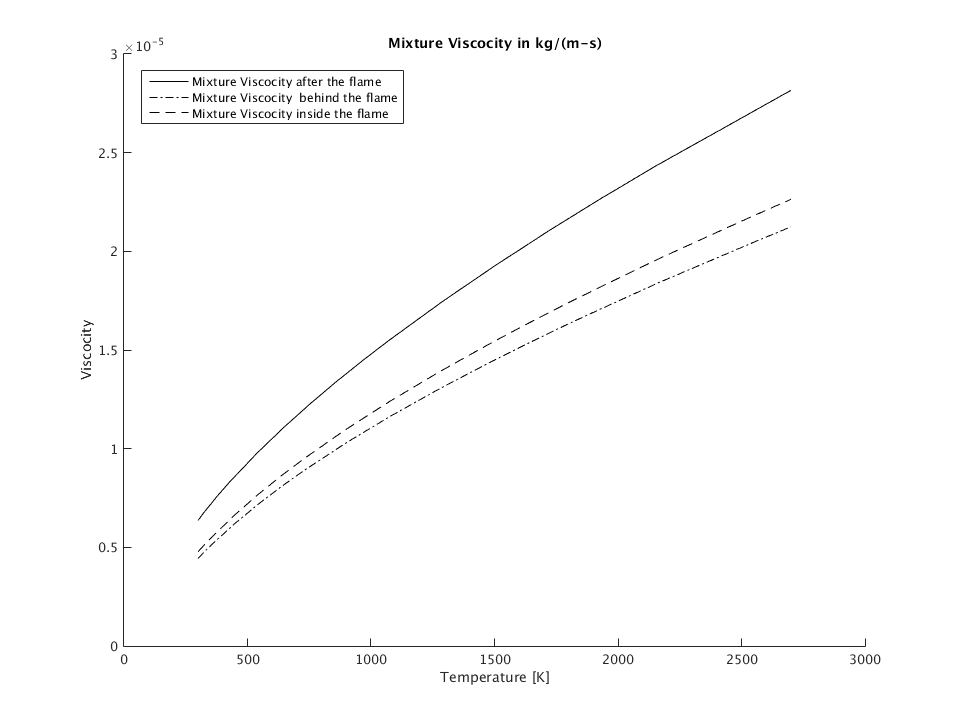
\includegraphics[scale=0.5]{figs/all_in_one.png}
%%     }

%%     \caption{Mixture Viscocity behind, inside, and after the flame}
%% \end{figure}


%%  For the bimolecular diffusion model, we use:
%% \begin{equation}
%% D_i = \frac{1-y_i}{\sum_{j\ne i}^{n}\frac{x_i}{D_{ji}}}
%%          = \frac{\sum_{j\neq i}^{n} x_j M_j}{M_{\textnormal{mixture}} \sum_{j\ne i}^{n}\frac{x_j}{D_{ji}}}
%% \end{equation}

%% \begin{figure}[H]

%% \subfloat[Mixture Diffusion coefficient for $O_3$ and $O_2$ \label{subfig-1:dummy}]{%
%%      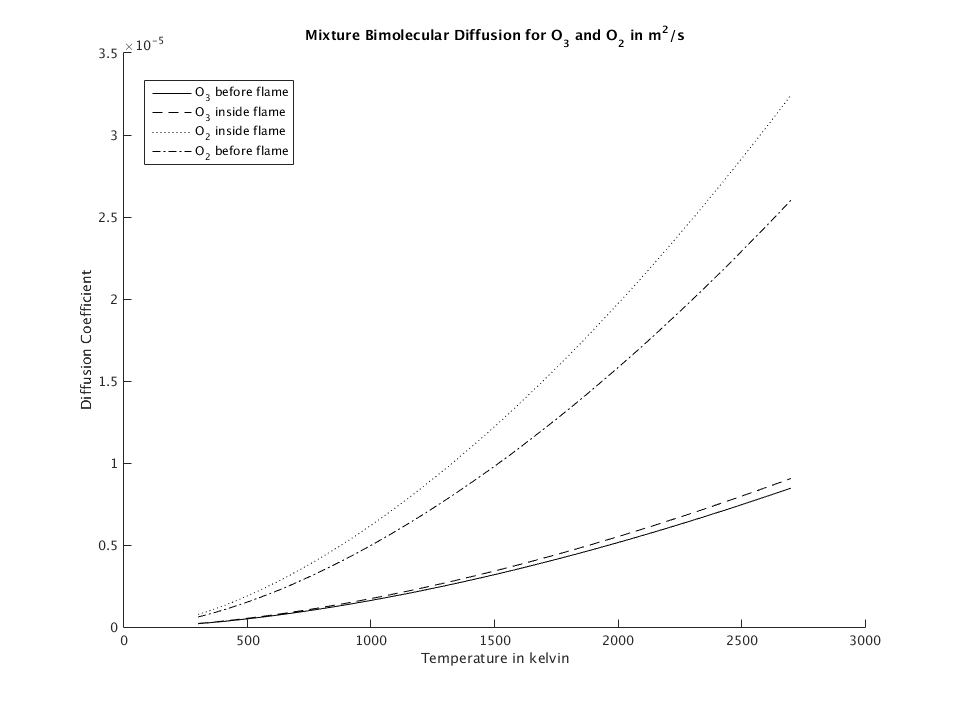
\includegraphics[scale=0.5]{figs/mixdiffusionO2O3.png}
%%     }
%%     \quad
%%   \subfloat[Mixture Diffusion coefficient for $O$ inside the flame\label{subfig-1:dummy}]{%
%%          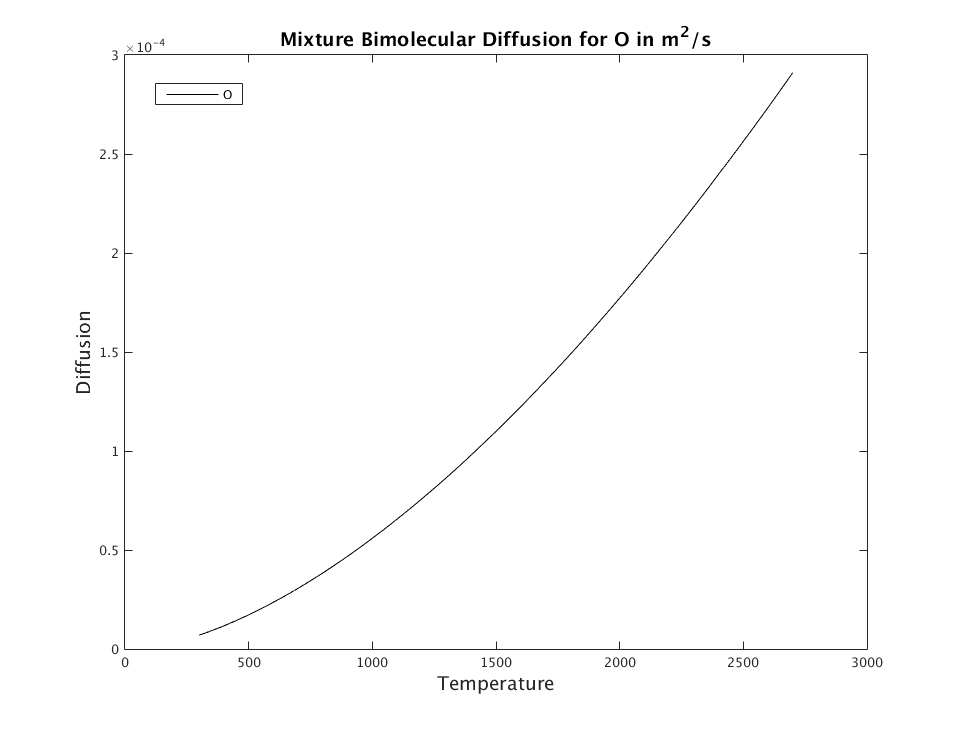
\includegraphics[scale=0.5]{figs/mixturediffusionO_inflame.png}
%%         }

%%     \caption{Mixture Diffusion coefficient}
%% \end{figure}


%%  The thermal conductivity of the mixture is given by Wilke rule\cite{Wilke}given by
%% \begin{equation}
%% \lambda_{\textnormal{mixture}} = \sum_{s=1}^{n} \frac {x_i \lambda_i}{\sum_{j=1}^{n} x_j \Phi_{ij}}
%% \end{equation}
%%   We have varied temperature from 300 K to 2700 K and plotted the mixture thermal conductivity V/s Temperature for all the  three species.  We have considered three cases-  behind the flame where condentration of $O_3$,$O_2$ and $O$ are taken to be .53, .47 and 0 respectively. Second case of the inside of the flame where concentrations are 0.5, 0.4 and 0.1 respectively. The third case is of the behind the flame where ozone and oxygen radical are absent and there will be only $O_2$. The $\sigma$ values and constants for dimensionless collision number are taken from GriMech 3.0\cite{gri}.


%% \begin{figure}[H]

%% \subfloat[Mixture thermal conductivity \label{subfig-1:dummy}]{%
%%      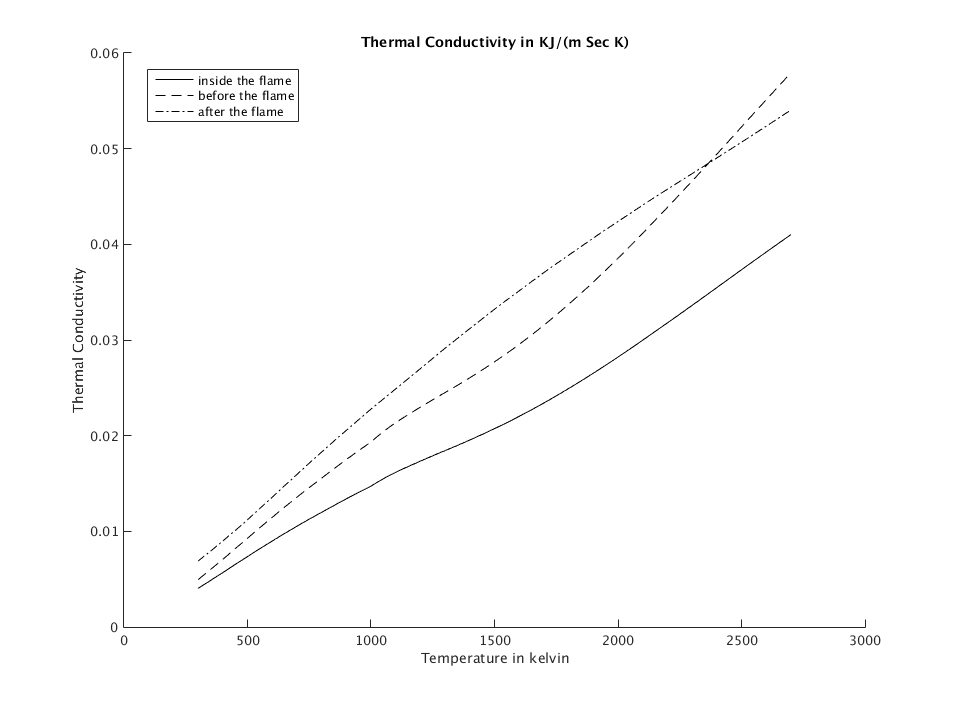
\includegraphics[scale=0.5]{figs/mixtherm.png}
%%     }

%%     \caption{Mixture thermal conductivity}
%% \end{figure}

%=======================================================================
% One-Dimensional Approximation
%=======================================================================
\section{One-Dimensional Approximation}\label{sec:1d}

It is common to use a one-dimensional approximation to predict
temperature and species profiles in a so-called ``free flame''
configuration. Thus, we affix the $x$-coordinate to the frame of the
flame and assume a steady state configuration. Then,
following~\cite{Smooke}, we have the following system of equations:
%
\begin{align}
  \dot{M} &= \rho u = \text{constant}\label{eq:mdot}\\
  \dot{M} \frac{dY_s}{dx} &= -\frac{d}{dx}\left( \rho Y_s V_s\right) +
  \dot{\omega}_s, \quad s=1,\dots,N_s \\
  c_p \dot{M} \frac{dT}{dx} &= \frac{d}{dx}\left( k \frac{dT}{dx}
  \right) - \frac{dT}{dx}\sum_{s=1}^{N_s} \rho Y_s V_s c_{p,s}  -
  \sum_{s=1}^{N_s} h_s \dot{\omega}_s \\
   p_0 &= \rho R T
\end{align}
%
where all quantities have been defined in
Section~\ref{sec:lowmach}.

Boundary conditions are specified at $x =
\pm \infty$. In particular,
%
\begin{align}
  T(-\infty) &= T_0 \\
  Y_s(-\infty) &= Y_{s,0}, \quad s = 1,\dots,N_s
\end{align}
%
and
%
\begin{align}
  \frac{dT}{dx}(\infty) &= 0 \\
  \frac{dY_s}{dx}(\infty) &= 0, \quad s = 1,\dots,N_s
\end{align}
%
Once $\dot{M}$ is computed, the flame speed can be directly calculated
using the inlet conditions to compute the density at the inlet.
Note that $\dot{M}$ is effectively an eigenvalue for this problem.
Theoretically, once could use, say, chemical equilibrium at
$x=\infty$, or zero derivatives at $x=-\infty$ to enforce
Equation~\eqref{eq:mdot}. Computationally, the condition is handled
differently in practice.

%%  The governing equations are givenin one dimensional and time dependent forms as follows from principles of combustion by Kuo.

%% The Overall continuity equation is given as
%% \begin{eqnarray}
%% \frac{\partial \rho}{\partial t} +  \frac{\partial \rho u }{\partial x} &= 0
%% \end{eqnarray}

%% The species continuity equation

%% \begin{eqnarray}
%% \rho \frac{Y_k}{\partial t} + \rho u \frac{Y_k}{\partial x} &= -\frac{\partial (\rho Y_k V_k)}{\partial x}  + w_k
%% \end{eqnarray}

%%  Where $k = 1, 2$ or  $3$ for $O$, $O_2$ or $O_3$ respectively.

%% Energy Equation

%% \begin{eqnarray}
%% \rho C_p \frac{\partial T}{\partial t} + \rho u C_p \frac{\partial T}{\partial x} &= \frac{\partial }{\partial x} \left(\lambda \frac{\partial T}{\partial x}\right)  - \sum_{k=1}^{N} w_k \Delta h^0_{fk} - \rho  \sum_{k=1}^{N} C_{p,k} Y_k V_k \frac{\partial T}{\partial x}
%% \end{eqnarray}

%%  This energy equations was arrived at under assumption that the pressure is constant in the reaction zone, the viscous dissipation is negligible, and there is no body force.

%%  The Diffusion equation is given as
%% \begin{eqnarray}
%% \frac{\partial X_k}{\partial x} &= \sum_{j=1}^{3} \frac{X_k X_j}{D_{jk}} (V_j - V_k)
%% \end{eqnarray}

%%  We have considered a free flame in a tube. In this configuration, there is a premixed mixture of fuel and oxidiser in given concentration. The spark is generated at a random point in the domain. The flae is developed anf it burns through the whole mixture untill all fuel is converted to oxygen. The boundary conditions for the totally burned end are

%% $$x \leftarrow \infty:  \frac{\partial T}{\partial x} = \frac{\partial Y_k}{\partial x} = 0$$

%%  In order to avoid solving the continuity equation along with the other equations, Heirmerl and coffee\cite{Heimerl} used a langrangian coordinate $\psi$
%% and a new time coordinate $\tau$ defined by

%% $$\psi \equiv \int_{0}^{x} \rho(x',t)dx'$$

%%  So by definiton of $\psi$ and by chain, we have these expressions
%%  $$\frac{\partial \psi}{\partial x} = \rho$$
%%  $$\frac{\partial \tau}{\partial x} = 0$$
%%  $$\frac{\partial \tau}{\partial t} = 1$$
%%  $$\frac{\partial \psi}{\partial t} = (\rho u)_{x=0} - (\rho u)_{x} $$

%%  By integrating the overall continuity equation from 0 to x, we obtain

%% $$\frac{\partial d}{\partial t} \int_{0}^{x} \rho dx + [(\rho u)_{x} - (\rho u)_{0} ] = 0$$

%%  The product $\rho u$ at $x =0$ is the eigenvalue of the problem. It is defined as

%% $$m_0 = (\rho u)_0$$

%%  The energy equation in the new coordinate system becomes

%% \begin{eqnarray}
%%  \frac{\partial T}{\partial t} + m_0 \frac{T}{\partial \psi} &= \frac{1}{C_p}\frac{d}{\partial \psi} \left(\rho \lambda \frac{\partial T}{\partial \psi}\right)  - \frac{1}{\rho C_p} \sum_{k=1}^{N} w_k \Delta h^0_{fk} - \frac{1}{C_p}  \sum_{k=1}^{N} C_{p,k} Y_k V_k \frac{\partial T}{\partial \psi}
%% \end{eqnarray}

%%  The eigenvalue of $m_0$ or $S_L$ was determined from the steady state solution of the problem, that is

%% $$\frac{\partial Y_k}{\partial t} = \frac{\partial T}{\partial t} = 0$$

%%  Under the steady state conditons,

%% $$\rho u = constant = \rho_\infty u_\infty = -\rho_1 S_L$$

\subsection{Numerical Approximation}

The first approximation is that the infinite domain is truncated to a
finite length, $x\in[0,L]$. $L$ must be sufficiently large to not
significantly influence the solution. Next, the boundary conditions
become
%
\begin{align}
  T(0) &= T_0 \\
  \varepsilon_s(0) &= Y_{s,0}, \quad s = 1, \dots, N_s
\end{align}
%
where $\varepsilon_s$ is the mass flux fraction of species $s$:
%
\begin{equation}
  \varepsilon_s = Y_s + \frac{\rho Y_s V_s}{\dot{M}}, \quad s = 1, \dots, N_s
\end{equation}
%
This condition is preferred for the inlet boundary condition to ensure
the proper mass flow since the domain has been truncated.
The outlet boundary conditions remain the same:
%
\begin{align}
  \frac{dT}{dx}(L) &= 0 \\
  \frac{dY_s}{dx}(L) &= 0, \quad s = 1, \dots, N_s
\end{align}
%
Finally, to treat the eigenvalue $\dot{M}$, an trivial auxillary
differential equation is introduced:
%
\begin{equation}
  \frac{d\dot{M}}{dx} = 0
\end{equation}
%
The choice made in~\cite{Smooke} is to specify the temperature at an
interior point:
%
\begin{equation}
  T(x_f) = T_f
\end{equation}
%
where $x_f$ and $T_f$ are user-specified parameters. Smooke et
al~\cite{Smooke} note that the convergence of the iterative procedure
can be particularly sensitive to these choices.

Following~\cite{Smooke}, the nonlinear boundary value problem is discretized using an upwind
finite difference approximation. The initial profiles are based on
cubic Hermite functions for temperature and major species and Gaussian
profiles for minor species; chemical equilibrium is used to provide
the initial guess for species post-flame. Newton's method with line
search~\cite{NocedalWright1999} is used to solve the resulting system
of nonlinear equations.

\subsection{Software Infrastructure}

The numerical scheme described previously has been deployed in the
Cantera software package~\cite{Cantera}. The Cantera C++ code provides
implementations for the thermodynamic, transport, and chemical
kinetics models described previously. Further, Cantera provides an
interface for computing solutions to the one-dimensional free flame
problem described previously. The only variation is that Cantera will
use simple time-stepping schemes to aid in obtaining a better initial
guess for the steady-state nonlinear solve. We have used Cantera
version 2.1.2 in this work.



 \section{Ozone Combustion Model} \label{sec:ozone-data}
We shall use Heimerl and coffee's\cite{Heimerl} contemporary method
for modelling combustion flame problem. A one dimensional, premixed,
laminar, steady state ozone oxygen flame was considered in their
theortical model. The reason for choosing this model was due to its
simplicity. The chemical reactions involve only three species:
%
\begin{equation}\label{eq:ozone-mech}
\begin{aligned}
  O_3 + M &\rightleftharpoons O + O_2 + M\\
  O + O_3 &\rightleftharpoons 2O_2\\
  2O + M &\rightleftharpoons O_2 + M
\end{aligned}
\end{equation}
%
Where M represents the third body which could be either $O$,
$O_2$ or $O_3$.



\subsection{Experimental Data}

Streng and Grosse~\cite{Streng} studied the ozone
flame experimentally. The stability of ozone and the rates of
decomposition or explosion were investigated.% by Armour research foundation.
Ozone was burned from a simple burner tip in the
range from 17 percent to 100 percent initial concentration of ozone in
the mixture.
%% The flame temperatures were calculated from enthalpy data
%% and dissociation constants of oxygen using kelley's tables.
The concentration of ozone was kept constant with error of 0.2
percent. Two methods were used to determine burning velocity i.e open
tube method and the burning tip method. We will be using experimental
burning velocity of the burning tip method. The burner tip experiments
were carried out in standard apparatus, using pyrex glass aluminium
tips with an inner diameter of 3 to 0.65mm. The flames were readily
observed by the standard schlieren method at all concentrations above
30 mole percent. The measurements were all carried out in the laminar
flow region and the reynolds number of the flow was below 2000. The
initial conditions are 300K temperature and 1.0 atmosphere
pressure. The results of burning velocities of ozone flames were
compared with theoretical burning velocities of Dr. Von Karman and his
associates. They were found to be in close agreements.


%%  To compare our results, we have used the experimental data
%% given by the A.G.  streng\cite{Streng} and A.V. Grosse, They have done
%% experiments with ozone flame in tube and ozone flame on the tip of the
%% burner. We will be using the results of the later. They have shown
%% that laminar flame speed or burning velocity varies with the initial
%% concentration of the ozone.

Table~\ref{tab:ozone-flame-data} shows the burning
velocity with respect to initial concentration of the ozone. We
concentrate on two speciifc cases where initial concentration of ozone
is 53 percent and 100 percent. The laminar flame speed for 53 percent
is measured in the burner with inner diameter 1.3mm and rate of 7.7
cc/sec. The laminar flame speed for 100 percent ozone is taken on .66
inner diameter tip 0.66 mm and the flow rate of 8.23 cc/sec.  The
measured laminar flame speed is given below. Laminar flame
measurements are carried out at 300K and 1 atmosphere pressure.

\begin{table}[h]
\caption {Experimental laminar flame speed given by A.G. Streng and
  A.V. Grosse\cite{Streng}} \label{tab:ozone-flame-data}
\begin{center}

\begin{tabular}{|c|c|}
\hline \textbf{ Initial Concentration of $O_3$ ($\pm 0.2 \% )$} &
\textbf{ Laminar Flame Speed (cm/s)} \\ \hline 17& 9.2 \\ \hline 20&
18.2 \\ \hline 28& 52.2 \\ \hline 40& 125 \\ \hline 46& 166 \\ \hline
53& 210 \\ \hline 75& 331 \\ \hline 100& 475 \\ \hline
\end{tabular}
\end{center}
\end{table}
